%!TEX root = ../dokumentation.tex
\chapter{Grundlagen und Stand der Forschung}

%https://www-ai.cs.tu-dortmund.de/PublicPublicationFiles/bierwirth_2018a.pdf

\section{Implementierungsumgebung Jupyter}
\par
Jupyter Notebooks ist eine von der non-profit Organisation Project Jupyter entwickelte Open-Source Lösung zur interaktiven Arbeit mit Dutzenden Programmiersprachen \cite{project_jupyter}. Der Name Jupyter leitet sich dabei von den drei primären Programmiersprachen Julia, Python und R ab. Jupyter Notebooks ist sprachunabhängig und unterstützt, unter Verwendung des IPython \gls{Kernel}, die Programmiersprachen Julia, R, Haskell, Ruby und Python \cite{jupyter_kernel}. Darüber hinaus werden unterschiedlichste Export Möglichkeiten wie \ac{HTML}, \ac{PDF} und \LaTeX \space unterstützt. Die in diesem Projekt verwendete Variante von Jupyter Notebooks ist Google Colab, eine speziell für die Python-Entwicklung entworfene Umgebung. Colab Notebooks führen Code auf Cloud-Servern aus und bieten somit unabhängige Vorteile gehosteter Hardware, wie \acp{GPU} und \acp{TPU} \cite{colab_notebooks}.

\section{Bildverarbeitungsalgorithmen mit OpenCV}

\section{Maschinelle Lernverfahren}

Maschinelle Lernverfahren lassen sich in drei Bereiche unterteilen. \citeauthor{Sejnowski1999} beschreibt in seinem Buch \citetitle{Sejnowski1999} das Unüberwachte Lernen \emph{(unsupervised learning)} als maschinelles Lernverfahren, das ohne zuvor bekannte Werte oder Belohnungen, Abweichungen vom strukturlosen Rauschen erkennt \cite{Sejnowski1999}. Ferner wird von \citeauthor{duda1973pattern} die automatische Segmentierung (Clustering) und die Komprimierung von Daten zur Dimensionsreduktion erwähnt, die zum fortwährenden Erfolg der Lernmethode beitragen \cites[51\psq]{duda1973pattern}[51\psq]{Cord2008}. Als eine weitere maschinelle Lernmethode führt \citeauthor{Cord2008} das Überwachte Lernen \emph{(supervised learning)} an. Das Überwachte Lernen beinhaltet das Lernen einer Abbildung zwischen einem Satz von Eingangsvariablen $X$ und einer Ausgangsvariablen $Y$, sowie die Anwendung dieser Abbildung zur Vorhersage der Ausgabe für ungesehene Daten \cite[21\psqq]{Cord2008}. \citeauthor{Cord2008} nennt \citeyear{Cord2008} als verbreitestes Modell die \ac{SVM}, die ihre Stärken besonders in der Verarbeitung von Multimedialen Daten besitzt. Im Paradigma des überwachten Lernens besteht das Ziel darin, eine Funktion $f:X \longrightarrow Y$ aus einem Beispiel- oder Trainingssatz $A_{n}$ abzuleiten \cite[22]{Cord2008}. Sei hierzu $x_i \in X$ und $y_i \in Y$:

\begin{equation}
	A_{n} = ((x_{1},y_{1}),\dots,(x_{n},y_{n})) \in (X \times Y)^{n}.
\end{equation}

Ein weiterer Fundamentaler Bestandteil des überwachten Lernens ist der Begriff des Verlusts zur Messung der Übereinstimmung zwischen der Vorhersage $f(x)$ und der gewünschten Ausgabe $y$. Hierfür wird eine Verlustfunktion $L:Y \times Y \longrightarrow \mathbb{R}^+$ zur Evaluierung des Fehlers eingeführt. Die Wahl der Verlustfunktion $L(f(x),y)$ hängt von dem zu lösenden Lernproblem ab \cite[22]{Cord2008}. 

Zu unterscheiden sind hierbei drei verschiedenen Arten - \emph{Binäre}, \emph{Multi-Class} sowie \emph{Multi-Label} Klassifikation. Für erstere ist es das Ziel, die Ausgabe eines messbaren zufälligen Klassifikators, parametrisiert durch $f:X\rightarrow [0,1]$, der zwischen positiven $(Y=1)$ und negativen $(Y=0)$ Instanzen unterscheidet, zu erzeugen \cite[2\psq]{pmlr-v81-menon18a}. Ein zufälliger Klassifikator sagt jedes $x \in X$ mit der Wahrscheinlichkeit $f(x)$ als positiv voraus; die Qualität eines solchen Klassifikators wird durch ein statistisches Risiko $R(\cdot;D): [0,1]^X \rightarrow \mathbb{R}_{+} $ bewertet \cite[3]{pmlr-v81-menon18a}. Die standardmäßig gewählte Verlustfunktion $L(f(x),y)$ für Binäre Klassifikation ist die Binäre Kreuzentropie (\emph{binary cross entropy}), definiert als

\begin{equation}
	CE = - \sum_{i=1}^{C'=2}{t_i \log(s_i) = -t_1 \log(s_1) - (1-t_1} \log(1-s_1).
\end{equation}

Es wird von zwei Klassen $C_1$ und $C_2$ ausgegangen. $t_1 \in [0,1]$ und $s_1$ sind die Grundwahrheit und der Wert für $C_1$; $t_2 = 1 - t_1$ sowie $s_2 = 1 - t_2$ für $C_2$ \cite{rubinstein2014cross}.

Sollte der vorgegebene Raum $[0,1]$ für die Klassifizierung nicht ausreichen, kann die \emph{Multi-Class Classification} eingesetzt werden. Hierfür wird die Binäre Klassifikation durch eine Auswahl verschiedener Strategien an das vorgegebene Lernproblem angepasst. Eine hierbei verwendete Methode ist die Transformation der Problemstellung in den binären Raum, welche mit Hilfe der \ac{OvR} oder \ac{OvO} Strategie umgesetzt werden kann. Die \ac{OvR}-Strategie beinhaltet dabei das Training eines einzelnen Klassifikators pro Klasse, wobei die Proben dieser Klasse als positive Proben und alle anderen Proben als negative Proben gelten. Diese Strategie erfordert, dass die Basisklassifikatoren einen realwertigen Konfidenzwert für ihre Entscheidung erzeugen und nicht nur ein Klassenetikett; diskrete Klassenetiketten allein können zu Mehrdeutigkeiten führen, bei denen mehrere Klassen für eine einzelne Probe vorhergesagt werden \cite[182]{Bishop2006}. Bei der \ac{OvO}-Strategie hingegen werden $K(K-1)/2$ binäre Klassifikatoren für ein $K$-Wege-Mehrklassenproblem trainiert. Jeder Klassifikator $K$ erhält die Proben eines Klassenpaares aus der ursprünglichen Trainingsmenge und muss lernen, diese beiden Klassen zu unterscheiden \cite[339]{Bishop2006}. Wie OvR leidet auch OvO unter Mehrdeutigkeiten, da einige Regionen des Eingaberaums die gleiche Anzahl von Stimmen erhalten können \cite[183]{Bishop2006}. 
Neben dem Einsatz der Transformation in den binären Raum, kann ein binärer Klassifikator auch zur Lösung von Mehrklassen Problemen erweitert werden. Aufgrund der Bedeutsamkeit dieser Anpassungstechnik in Kontext dieser Arbeit, wird hierauf in Kapitel \ref{sec:ann} tiefer eingegangen.


%Weiterführend wird hierauf in Kapitel \ref{sec:optimize} eingegangen.

\subsection*{Optimierungsverfahren für maschinelle Lernmethoden}\label{sec:optimize}

Damit eine Vielzahl von optimalen Lösungen für verschiedene Fragestellungen ermittelt werden kann, kommen Optimierungsverfahren zum Einsatz. Der Grundgedanke dieser ist es, die Parameter iterativ so zu verändern, dass eine Kostenfunktion minimiert wird.

\subsubsection{Gradientenverfahren}
Das Gradientenverfahren ist anwendbar, um eine differenzierbare Funktion $f:\mathbb{R}^n \rightarrow\mathbb{R}$ mit einem reellen Wert zu erhalten, die minimiert werden soll:

\begin{equation}
	\min_{x\in\mathbb{R}^n} f(x).
\end{equation}

Das Verfahren berechnet den lokalen Gradienten der Fehlerfunktion, entsprechend dem Parametervektor $\theta$ und bewegt sich in Richtung eines abnehmenden Gradienten. Sobald die Steigung Null annimmt, ist ein Minimum erreicht. Zu Beginn wird $\theta$ mit Zufallszahlen initialisiert, welche anschließend in kleinen Schritten verbessert werden um die Kostenfunktion\footnote{Als Kostenfunktion kann z.B. der \ac{MSE} eingesetzt werden.} zu senken. Dieser Schritt wird wiederholt, bis der Algorithmus bei einem lokalen Minimum konvergiert \cite[112\psq]{Géron2017} (siehe Abbildung \ref{fig:gradient_descent}). 

\begin{figure}[htbp]
	
	\usetikzlibrary{arrows.meta}
	\centering
	\tikzset{
  		point/.style = {% define a style for the function points
    	circle,
    	fill=#1,
    	draw=black,
    	inner sep=2pt,
  	},
  	point/.default = {green!60}
	}

	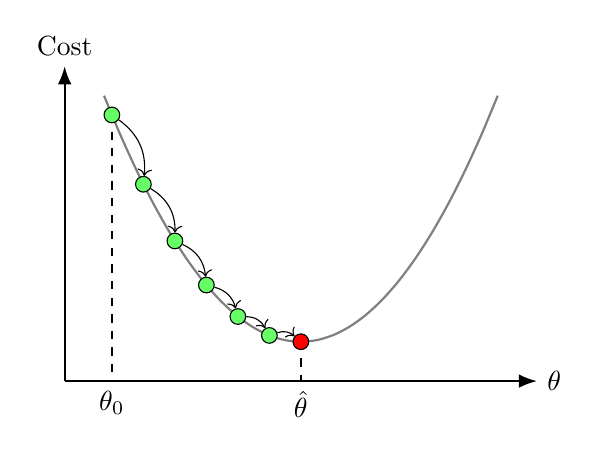
\begin{tikzpicture}[declare function={f(\x)=0.5*\x*\x-3*\x+5;}]
    	\draw[thick,-{LaTeX}](0,0)--(6,0) node[right]{$\theta$};
    	\draw[thick,-{LaTeX}](0,0)--(0,4) node[above]{Cost};
    	\draw[thick, dashed](0.6, {f(0.6)}) -- (0.6,0)
       	   node[below, text width=4em, align=center]{$\theta_0$};
    	\draw[thick, dashed](3, {f(3)}) -- (3,0) node[below]{$\hat\theta$};
    	\draw[domain=0.5:5.5, smooth, thick, gray] plot (\x, f(\x);
    	\foreach \a [count=\c, remember=\c as \C] in {0.6, 1.0, ..., 2.6} {
      	\node[point] (\c) at (\a, {f(\a)}){};
      	\ifnum\c>1 % after the first coordinate draw an arrow
        	 \draw[->, bend left](\C) to (\c);
      	\fi
    	}
    	\node[point=red] (Y) at (3, {f(3)}){}; % add the yellow point
    	\draw[->, bend left](6) to (Y);
 	\end{tikzpicture}
 	\caption{Gradientenverfahren mit zufälligem Startvektor $\theta_0$ und lokalem Minimum $\hat\theta$}
 	\label{fig:gradient_descent}
\end{figure}

Bei der iterativen Suche eines Minimums ist dabei die Schrittgröße zu beachten. Diese wird durch die zuvor definierte Lernrate ermittelt, die als \gls{Hyperparameter} der Gleichung anzusehen ist. Ist die Lernrate zu klein, steigen die Schritte des Algorithmus, was ihn langsam und ineffizient werden lässt. Eine zu große Lernrate kann hingegen zur Divergenz des Algorithmus führen \cite[114]{Géron2017}.


\section{Datenstromorientierte Programmierung mit TensorFlow}
%TensorFlow ist eine Open-Source Bibliothek für das Maschinelle Lernen und wird seit 2017 von Google angeboten. Es wurde vom Google Brain Team entwickelt und ermöglicht es dank zahlreicher \acp{API} Deep-Learning Aufgaben effizient zu lösen. Seit Ende 2019 ist TensorFlow 2 mit der Integration von Keras verfügbar. Der Kern von TensorFlow ist in der Programmiersprache C++ implementiert und ermöglicht die Ausführung von Operationen auf verschiedenen Hardwareplattformen (CPU, GPU und TPU) und Betriebssystemen. Parallel dazu wurde zur Verbesserung der Ausführungszeiten und Speicheroptimierung \ac{XLA} entwickelt, ein Compiler, der spezifische mathematische Funktionen für TensorFlow optimiert und sie hardwareunabhängig ausführen kann.

TensorFlow ist eine Open-Source-Bibliothek für maschinelles Lernen, die von Google seit 2017 angeboten wird. Sie wurde vom Google Brain Team entwickelt und ermöglicht dank vieler \acp{API} Deep-Learning, um Aufgaben effizient zu lösen. Seit Ende 2019 ist TensorFlow 2 mit Keras-Integration verfügbar. Der Kern von TensorFlow ist in der Programmiersprache C++ implementiert und ermöglicht die Ausführung von Operationen auf unterschiedlichen Hardware-Basen (\acs{CPU}, \ac{GPU} und \ac{TPU}) und Betriebssystemen.  Parallel dazu wurde zur Verbesserung der Ausführungszeiten und der Speicheroptimierung \ac{XLA} entwickelt, ein Compiler, der spezifische mathematische Funktionen für TensorFlow optimiert und diese unabhängig von der Hardware ausführen kann \cite[139\psq]{Deru2019}.

\begin{figure}[ht]
	\centering
	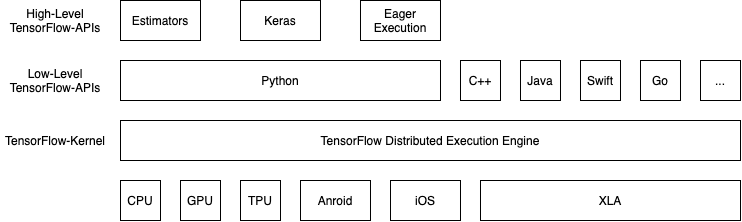
\includegraphics[width=\textwidth]{images/TF2-API-Struktur}
	\caption[TensorFlow API Struktur]{API-Struktur von TensorFlow 2 (grafisch adaptiert von \cite[140]{Deru2019}\cites{TfAPI})}
	\label{fig:tfstructure}
\end{figure}

\subsection{Tensoren}
Grundlegender Bestandteil TensorFlows sind die schon im Namen enthaltenen Tensoren. Sie werden primär zur Datenspeicherung in neuronalen Netzen eingesetzt. 

\subsection{Künstliche neuronale Netze}\label{sec:ann}

Die Ursprünge der künstlichen neuronalen Netze lassen sich auf \citeauthor{mcculloch_pitts} im Jahre \citeyear{mcculloch_pitts} zurückführen \cite{mcculloch_pitts}. Eine von Donald O. Hebb 1949 formulierte Lernregel stellt seither in ihrer allgemeinen Form die Grundlage der künstlichen neuronalen Lernverfahren dar \cite{Mainzer1997}. Ein künstliches neuronales Netz besteht aus einer Eingabeschicht von Neuronen, $1..n$ versteckter Schichten und einer letzten Schicht von Ausgangsneuronen. Ein einzelnes Neuron nimmt überlicherweise mehrere Werte $x_{1},...,x_{n}$ und einen \gls{Bias}-Term $w_{0}$ als Eingabe und berechnet daraus die Ausgabe $y=h(z)$.

\begin{figure}[ht]
	\centering
	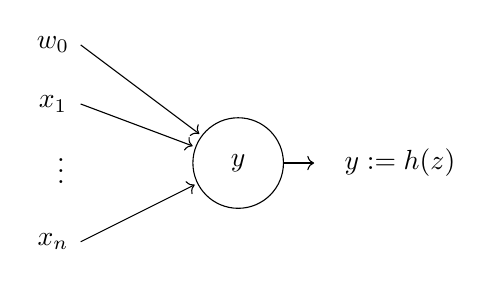
\begin{tikzpicture}[shorten >=1pt,->]
		\tikzstyle{unit}=[draw,shape=circle,minimum size=1.15cm]
 
		\node[unit](p) at (2,1){$y$};
		\node(dots) at (-0.25,1){\vdots};
 
		\draw (0,2.5) node[xshift=-10]{$w_0$} -- (p);
		\draw (0,1.75) node[xshift=-10]{$x_1$} --(p);
		\draw (0,0) node[xshift=-10]{$x_n$} -- (p);
		\draw (p) -- (3,1) node[xshift=30]{$y := h(z)$};
	\end{tikzpicture}
	\caption[Einzelnes Neuron mit dessen Komponenten]{Einzelnes Neuron mit dessen Eingangsvariablen. Die Aktivierungsfunktion ist beschrieben als $h$ und wird auf die tatsächlichen Eingabe $z$ angewandt. $x_1 ,..., x_n$ repräsentieren die Eingabe von anderen Neuronen innerhalb des Netzes. $w_0$ wird \gls{Bias} genannt und repräsentiert ein externes Gewicht \cite{stutz_neural_networks}.}
	\label{fig:processing-unit}
\end{figure}

Die Ausgabe $h_{i}$ des Neurons $i$ in der versteckten Schicht wird beschrieben durch

\begin{equation}
	h_{i} = \varphi(\sum_{j=1}^N{V_{ij}x_{j}+\theta_{i}^{hid}})
\end{equation}

wo $\varphi(\cdot)$ die Aktivierungsfunktion, $N$ die Anzahl der Eingangsneuronen, $V_{ij}$ die Gewichte, $x_{j}$ die Eingabe zum Neuron und $\theta_{i}^{hid}$ der Schwellenwertterm der versteckten Neuronen ist \cites[81-100]{Wang2003}[195-201]{Networks1995}. Die Intention der Aktivierungsfunktion $\varphi(\cdot)$ neben der Einführung von Nichtlinearität in das neuronale Netz ist, den Wert eines Neurons zu begrenzen, damit das neuronale Netz nicht durch divergierende Neuronen gelähmt wird. Eine gängige Aktivierungsfunktion ist die Sigmoid Funktion $\sigma(\cdot)$, wie definiert in \ref{eq:sigmoid}.

\begin{equation}\label{eq:sigmoid}
	\sigma(u) = \frac{1}{1 + e^{-u}}
\end{equation}


Weitere sigmoide Aktivierungsfunktionen sind der Arkustangens ($\arctan$) und Tangens Hyperbolikus ($\tanh$) \cite[195-201]{Networks1995}. Sie haben ein ähnliches Ansprechverhalten auf die Eingangswerte wie die Sigmoidfunktion, unterscheiden sich aber in den Ausgangsbereichen. 

\begin{figure}[htb]
\centering
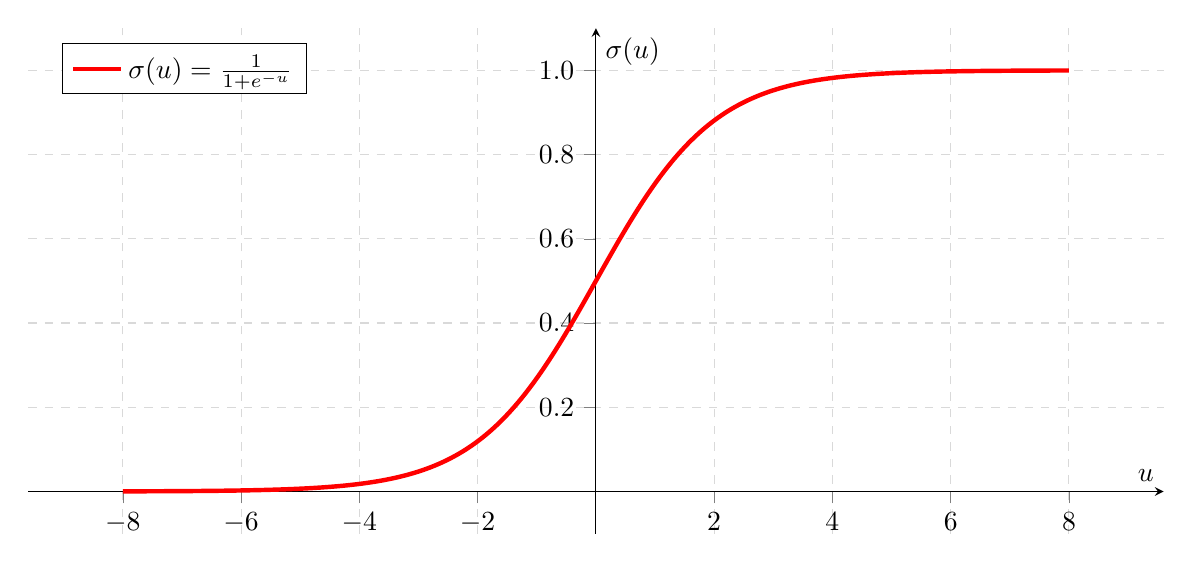
\begin{tikzpicture}\label{fig:sigmoid}
    \begin{axis}[
        legend pos=north west,
        axis x line=middle,
        axis y line=middle,
        y tick label style={/pgf/number format/fixed,
                            /pgf/number format/fixed zerofill,
                            /pgf/number format/precision=1},
        grid = major,
        width=16cm,
        height=8cm,
        grid style={dashed, gray!30},
        xmin=-8,     % start the diagram at this x-coordinate
        xmax= 8,     % end   the diagram at this x-coordinate
        ymin= 0,     % start the diagram at this y-coordinate
        ymax= 1,     % end   the diagram at this y-coordinate
        %axis background/.style={fill=white},
        xlabel=$u$,
        ylabel=$\sigma(u)$,
        tick align=outside,
        enlargelimits=true]
      % plot the stirling-formulae
      \addplot[domain=-8:8, red, ultra thick,samples=500] {1/(1+exp(-1*x))};
      \addlegendentry{$\sigma(u)=\frac{1}{1+e^{-u}}$}
    \end{axis}
\end{tikzpicture}
\caption{Darstellung der Sigmoid Aktivierungsfunktion}
\end{figure}

\subsection{Convolutional Neural Networks}

Seitdem \gls{AlexNet} im Jahre 2012 eine Auszeichnung beim jährlichen Wettbewerb der Benchmark-Datenbank ImageNet erzielte \cite{imagenet}, hat sich der Forschungsfokus auf das Themengebiet \emph{Deep Learning} zubewegt \cites{NIPS2012_c399862d, rastegari2016xnornet, russakovsky2015imagenet}. Zuvor waren \acp{SVM} der prävaliernde Ansatz zur Erkennung von Mustern.

\acp{CNN} werden seit 1995 in der digitalen Bildverarbeitung eingesetzt und sind fester Bestandteil des \emph{Deep Learnings}. Es werden Faltmatrizen der Größe 3x3, 5x5, 7x7 bzw. 9x9 eingesetzt, um Bereiche der Eingabematrix sukzessiv zu analysieren. Die dabei verwendeten \emph{convolutional operations} (Faltoperationen) erzeugen rezeptive Felder, die eine Merkmalskarte (\emph{feature map}) des \ac{CNN} generieren \cite{russakovsky2015imagenet}. Die rezeptiven Felder korrespondieren mit einer Region aus dem Originalbild \cite{Yan2020}. 
% Begin Figure CNN Matrix
\usetikzlibrary{matrix,positioning}
\begin{figure}[htb]
\centering
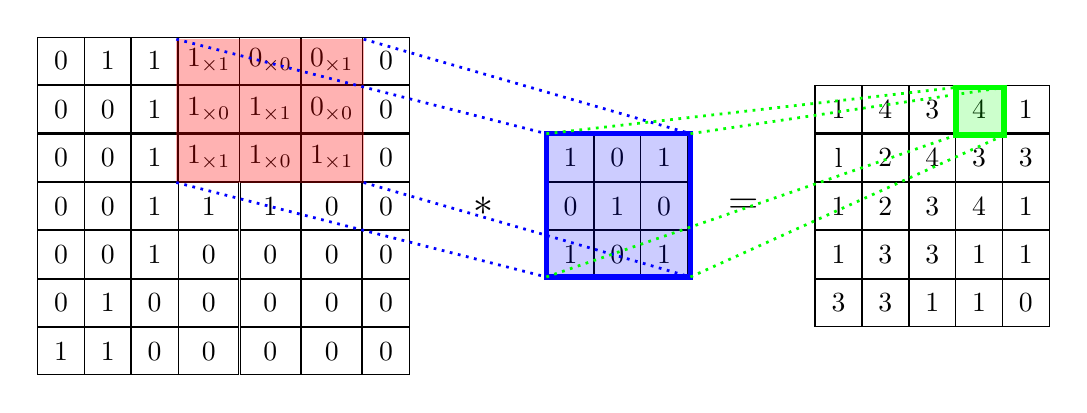
\begin{tikzpicture}[scale=1.0]

  \matrix [nodes=draw,column sep=-0.2mm, minimum size=6mm]
  {
    \node {0}; & \node{1}; & \node {1}; & \node{$1_{\times 1}$}; & \node{$0_{\times 0}$}; 
    & \node{$0_{\times 1}$}; & \node{0}; \\
    \node {0}; & \node{0}; & \node {1}; & \node{$1_{\times 0}$}; & \node{$1_{\times 1}$}; 
    & \node{$0_{\times 0}$}; & \node{0}; \\
    \node {0}; & \node{0}; & \node {1}; & \node{$1_{\times 1}$}; & \node{$1_{\times 0}$}; 
    & \node{$1_{\times 1}$}; & \node{0}; \\
    \node {0}; & \node{0}; & \node {1}; & \node{\, 1 \,}; & \node{\, 1 \, }; 
    & \node{\, 0 \,}; & \node{0}; \\
    \node {0}; & \node{0}; & \node {1}; & \node{\, 0 \, }; & \node{\, 0 \, }; 
    & \node{\, 0 \,}; & \node{0}; \\
    \node {0}; & \node{1}; & \node {0}; & \node{\, 0 \, }; & \node{\, 0 \, }; 
    & \node{\, 0 \,}; & \node{0}; \\
    \node {1}; & \node{1}; & \node {0}; & \node{\, 0 \,}; & \node{\, 0 \, }; 
    & \node{\, 0 \,}; & \node{0}; \\
  };


  % coordinates for coloring filter in array
  \coordinate (A) at (-0.6,0.3);
  \coordinate (B) at (1.78,0.3);
  \coordinate (C) at (1.78,2.12);
  \coordinate (D) at (-0.6,2.12);
  \fill[red, opacity=0.3] (A)--(B)--(C)--(D)--cycle;
  \begin{scope}[shift={(3.3,0)}]
    \node[] at (0,0) {\Large $\ast$};
  \end{scope}[shift={(2.5,0)}]

  \begin{scope}[shift={(5,0)}]

    %\matrix [matrix of math nodes,left delimiter={[},right
    %delimiter={]}]
    \matrix [nodes=draw,column sep=-0.2mm, minimum size=6mm]
    {
      \node{1};  & \node{0};   & \node{1};  \\
      \node{0};  & \node{1};   & \node{0};  \\
      \node{1}; & \node{0}; & \node{1}; \\
    };
    \coordinate (A1) at (-0.9,-0.9);
    \coordinate (B1) at (0.93,-0.9);
    \coordinate (C1) at (0.93,0.92);
    \coordinate (D1) at (-0.9,0.92);
    \fill[blue, opacity=0.2] (A1)--(B1)--(C1)--(D1)--cycle;
    \draw[blue, line width=2] (A1)--(B1)--(C1)--(D1)--cycle;
  \end{scope}

  \draw[dotted, line width=1, color=blue] (A)--(A1);
  \draw[dotted, line width=1, color=blue] (B)--(B1);
  \draw[dotted, line width=1, color=blue] (C)--(C1);
  \draw[dotted, line width=1, color=blue] (D)--(D1);

  \begin{scope}[shift={(6.6,0)}]
    \node[] at (0,0) {\Large $=$};
  \end{scope}[shift={(2.5,0)}]

  \begin{scope}[shift={(9,0)}]

    %\matrix [matrix of math nodes,left delimiter={[},right
    %delimiter={]}]
    \matrix [nodes=draw,column sep=-0.2mm, minimum size=6mm]
    {
      \node{1};  & \node{4};   & \node{3}; & \node{4}; & \node{1};  \\
      \node{l};  & \node{2};   & \node{4}; & \node{3}; & \node{3};  \\
      \node{1}; & \node{2}; & \node{3}; & \node{4} ; & \node{1};  \\
      \node{1}; & \node{3}; & \node{3}; & \node{1} ; & \node{1};  \\
      \node{3}; & \node{3}; & \node{1}; & \node{1} ; & \node{0};  \\
    };
    \coordinate (A2) at (0.3,0.9);
    \coordinate (B2) at (0.91,0.9);
    \coordinate (C2) at (0.91,1.507);
    \coordinate (D2) at (0.3,1.507);
    \fill[green, opacity=0.2] (A2)--(B2)--(C2)--(D2)--cycle;
    \draw[green, line width=2] (A2)--(B2)--(C2)--(D2)--cycle;
  \end{scope}

  \draw[dotted, line width=1, color=green] (A1)--(A2);
  \draw[dotted, line width=1, color=green] (B1)--(B2);
  \draw[dotted, line width=1, color=green] (C1)--(C2);
  \draw[dotted, line width=1, color=green] (D1)--(D2);
\end{tikzpicture}
\caption{Erzeugen einer Merkmalskarte durch schrittweise Faltung}
\end{figure}


In der Mathematik wird die Faltung als eine Operation auf zwei Funktionen $f,g$ beschrieben, die eine dritte Funktion $f * g$ erzeugt. Die dritte Funktion beschreibt, wie die Form von $f$ durch $g$ verändert oder gefiltert wird. Für eine Position $ z_{ i,j } $ in der Ausgabe gilt

\begin{equation}
	z_{i,j}=b+\sum_{u=0}^{f_{h}-1}\sum_{v=0}^{f_{w}-1}{x_{i+u,j+v}\cdot w_{u,v}}
\end{equation}

worin $z_{i,j}$ die Position innerhalb der Matrix $z$ beschreibt und $b$ der \gls{Bias} ist \cite[6]{karl2020}. Betrachtet man nun die Position $z_{i,j}$ in der Ausgabe eines Layers gilt 

\begin{equation}
	z_{i,j}=b+\sum_{u=0}^{f_{h}-1}\sum_{v=0}^{f_{w}-1}{x_{i',j'}\cdot w_{u,v}}\text{  \space\space\space    } \begin{cases}
	i' = i \cdot s_{h} + u \\ j' = j \cdot s_{w} + v 
\end{cases}
\end{equation}

worin $s_h$ der vertikale und $s_w$ der horizontale Stride sind \cite[13\psq]{karl2020}. Der Stride ist eine Komponente des \ac{CNN}, abgestimmt auf die Kompression des Eingabedatensatzes. Weitergehend wird er als Parameter des \ac{CNN}-Filters bezeichnet, der die Bewegung  über die Eingabematrix bestimmt.

Die darauffolgende \emph{Volume Convolution} erweitert die Gleichung um einen Parameter $k$ , der die Anzahl der Farbräume in die Gleichung einbezieht \cites[25]{karl2020}[365]{Géron2017}. Es gilt
	
\begin{equation}
	z_{i,j,k'}=b_{k'}+\sum_{c=1}^k{}\sum_{u=0}^{f_{h}-1}\sum_{v=0}^{f_{w}-1}{x_{i',j',c}\cdot w_{u,v,c,k'}}\text{  \space\space\space    } \begin{cases}
	i' = i \cdot s_{h} + u \\ j' = j \cdot s_{w} + v 
\end{cases}
\end{equation}
Die Anzahl der Parameter eines \ac{CNN} ist unabhängig von der Eingabe, jedoch abhängig von der Größe des Filters \cite[28]{karl2020}. Allgemein gilt daher 

\begin{equation}
	\text{\#{ }Params}_{conv} = (f_{w} \cdot f_{h} \cdot k^{l-1} + 1) \cdot k^l
\end{equation}

\section{Deep Learning mit Keras}

\section{Verwandte Arbeiten}
Der Einsatz maschineller Lernmethoden zur Erkennung von Objekten im Straßenverkehr ist weit verbreitet.
Es existieren bereits mehrere Arbeiten, die sich mit der intelligenten Erkennung von Objekten im Straßenverkehr befassen. Ziel ist dabei, Rückschlüsse zu unterschiedlichsten Situationen zu erlangen, zum Beispiel der Verkehrsoptimierung innerhalb von Großstätten oder der Erkennung von Geschwindigkeitsüberschreitungen.

Die Arbeit \cite{Atkočiūnas_Blake_Juozapavičius_Kazimianec_2005} beschreibt eine Möglichkeit, die Überwachung von Verkehrsflüssen zur Analyse des Straßenverkehrs, mit Hilfe von Bildverarbeitungs- und Mustererkennungsmethoden umzusetzen. Die dabei verwendeten Methoden ergeben die Funktionalität des Systems zur Überwachung der Straße sowie der Messung von Geschwindigkeiten. Zusätzlich werden die Nummernschilder der Fahrzeuge erfasst.


In der Arbeit \cite{9148964} werden parametrische sowie nicht-parametrische Methoden zur Vorhersage von Verkehrsaufkommen als wichtiger Teil des intelligenten Verkehrssystems (ITS) analysiert. Dabei wird die Berücksichtigung nichtlinearer Merkmale in maschinellen Lernmethoden analysiert und der Implementierungsaufwand in Bezug auf den Zeitaufwand für Training und Vorhersage gegenübergestellt. Darüber hinaus wurde eine Optimierungsmethode entwickelt um die Skalierbarkeit bestimmter Modelle zu verbessern.

Eine weitere Arbeit \cite{ata2019modelling} nimmt das dramatische Wachstum der Bevölkerung in Großstädten als Motivation zur Entwicklung effizienter Verkehrssysteme. Der darin erwähnte dynamische Verkehrsfluss erfordert einen Mechanismus zur Vorhersage von Verkehrsstaus mit Hilfe künstlicher Neuronaler Netze. Der entwickelte Mechanismus soll die entstandenen Staus kontrollieren bzw. minimieren und zu einer Beruhigung des Straßenverkehrs führen. Die Autoren verwenden einen Backpropagation-Algorithmus zum Trainieren des Neuronalen Netzes und der daraus hervorkommenden Lösung zum Treffen intelligenter Entscheidungen in der Verkehrssteuerung.

In der Arbeit \cite{devi2017machine} werden \ac{IOT}-Sensoren innerhalb eines Smart-City Szenarios eingesetzt, um Daten für eine Analyse des Verkehrsflusses unter Verwendung neuronaler Netze zu sammeln. Die dabei generierte Verkehrsstauvorhersage wird für die Analyse des Verkehrs sowie der Vorhersage von Staus auf bestimmten Strecken eingesetzt.

In Abgrenzung zu den genannten Arbeiten wird in dieser Arbeit ein \ac{CNN} dazu eingesetzt, Verkehrsobjekte zu erkennen und eine aussagekräftige Statistik zu erzeugen.


